% !TEX root =  ../appendix.tex

\section{Joint Model for the Kidney Transplant Dataset}
\label{sec : jm_amctx}
A total of 239 kidney transplant patients were included in the data set. The transplantation characteristics of these patients is presented in Table \ref{tab : baseline_characteristics}. The data set also includes periodical measurements of SCr and PCR. Our goal is to check if SCr and PCR both, are useful to predict graft failure. To this end, we model the two longitudinal outcomes and graft failure together using the joint modeling framework described in \ref{sec : jm_framework}. In this model we use log transformed values of both SCr and PCR \citep{fournier2016joint}. More specifically, we model the impact of log(SCr) value and log(SCr) velocity, log(PCR) value and log(PCR) velocity, and transplantation characteristics on the hazard of graft failure. In this regard, the JM consists of a multivariate longitudinal sub-model to model the evolution of SCr and PCR and a relative risk sub-model to model the impact of transplantation characteristics and biomarkers on the hazard of graft failure. The longitudinal evolution of the two outcomes over time is modeled flexibly using B-splines. The model formulation for PCR outcome is as follows (for SCr outcome it is similar):
\begin{equation}
\label{eq : long_model_prias}
\begin{aligned}
\log \mbox{PCR}(t) &= \beta_0 + \beta_1 \mbox{rec\_age} + \beta_2 \mbox{d\_age} + \beta_3 \mbox{d\_bmi} + \beta_4 \mbox{rec\_bmi} + \beta_5 \mbox{cit}\\
&+ \beta_6 \mbox{hla} + \beta_7 \mbox{pra}+ \beta_8 \mbox{dial\_days} + \beta_9 \mbox{ah\_nr} + \beta_{10} \mbox{rec\_gender} + \beta_{11} \mbox{d\_gender} \\
&+ \beta_{12} \mbox{dgf} + \beta_{13} \mbox{prev\_tp} + \beta_{14} \mbox{dm} + \beta_{15} \mbox{hvdis}+ \beta_{16} \mbox{d\_cadaveric}\\
&+\sum_{k=1}^4 \beta_{k+16} B_k(t,\mathcal{K}) +  b_{i0} + \sum_{k=1}^4 b_{ik} B_k(t,\mathcal{K}) + 
\varepsilon_i(t),
\end{aligned}
\end{equation}
where $B_k(t, \mathcal{K})$ denotes the $k$-th basis function of a B-spline with three internal knots at $\mathcal{K} =\{0.082, 0.219, 1\}$ (30 and 80 days) years, and boundary knots at 0.039 and 6 years (minimum and 0.95 quantile of the time of measurements two outcomes). The abbreviated covariate names correspond to the covariates in Table \ref{tab : baseline_characteristics}. The quantitative transplantation characteristics are standardized to avoid convergence issues in parameter estimation. For the relative risk sub-model the hazard function we fit is given by:
\begin{equation}
\label{eq : hazard_prias}
\begin{aligned}
h_i(t) &= h_0(t) \exp\big\{\gamma_1 \mbox{prev\_tp} + \gamma_2 \mbox{hla}  + \gamma_3 \mbox{cit} + \gamma_4 \mbox{dial\_days} \\
& + \alpha_{11} m_{i1}(t) + \alpha_{12} m'_{i1}(t) + \alpha_{21} m_{i2}(t) + \alpha_{22} m'_{i2}(t)\big\},
\end{aligned}
\end{equation}
where $\alpha_{11}, \alpha_{12}, \alpha_{21}$ and $\alpha_{22}$ are measures of strength of the association between hazard of graft failure and $\log \mbox{PCR}$ value $m_{i1}(t)$, $\log \mbox{PCR}$ velocity $m'_{i1}(t)$, $\log \mbox{SCr}$ value $m_{i2}(t)$ and $\log \mbox{SCr}$ velocity $m'_{i2}(t)$ respectively.

The parameters of the JM are estimated using the R package \textbf{JMbayes} \citep{rizopoulosJMbayes}, which uses the Bayesian methodology to estimate the model parameters. The parameter estimates for the relative risk sub-model are provided in Table \ref{tab : relative_risk}. Since the quantitative variables are standardized, the effect sizes correspond to one standard deviation increase in the corresponding variable.  The parameter estimates for the longitudinal sub-model for SCr and PCR are provided in Table \ref{tab : creatinine_long} and Table \ref{tab : pcr_long}, respectively. To avoid the tricky interpretation of variables corresponding to evolution over time, instead the evolution of SCr and PCR over time is depicted in Figure \ref{fig : creatinine_evolution}, and Figure \ref{fig : pcr_evolution}, respectively.

\begin{table}[!htb]
\begin{center}
\caption{Observed transplantation characteristics of the studied population (n = 239).}
\label{tab : baseline_characteristics}
\begin{tabular}{llr}
\Hline
\multicolumn{3}{c}{Quantitative characteristics} \\
\hline
Name & Abbreviation & Mean (SD) \\ 
\hline
Receiver age (at baseline) & rec\_age & 50.70 (13.09) \\
Donor age & d\_age & 49.73 (12.66) \\
Donor BMI & d\_bmi & 25.10 (4.43) \\
Receiver BMI & rec\_bmi & 25.43 (4.31) \\
Cold ischemia time (minutes) & cit & 887.25 (522.95)\\
\#HLA A, B and DR mismatches & hla & 2.81 (1.57)\\
Panel reactive antibody (\%) & pra & 4.81 (14.20) \\
\#Days on dialysis before transplant & dial\_days & 1334.91 (1283.93)\\
\#Anti-hypertensive medicaments & ah\_nr & 1.58 (0.96)\\
\hline
\\
\multicolumn{3}{c}{Categorical characteristics}\\
\hline
Name & Abbreviation & Category (\%) \\
\hline
Receiver gender & rec\_gender & Female (42.68 \%)\\
Donor gender & d\_gender & Female (56.49 \%)\\
Delayed graft function after transplant & dgf & No (67.78 \%)\\
Previous transplantation & prev\_tp & No (84.45 \%)\\
Diabetes mellitus & dm & No (84.52 \%)\\
Known cardiovascular events before transplant & hvdis & No (61.92 \%)\\
Deceased donor & d\_cadaveric & No (25.94 \%)\\
\hline     
\end{tabular}
\end{center}
\end{table}

\begin{table}[!htb]
\begin{center}
\caption{Parameter estimates for the relative risk sub-model for the log hazard and 95\% credible interval.}
\label{tab : relative_risk}
\begin{tabular}{lrrrrr}
\Hline
Variable               & Mean   & Std. Dev & 2.5\%  & 97.5\% & P              \\
\hline
Previous transplant: Yes      & 0.305  & 0.339    & -0.099 & 0.986  & 0.352          \\
\#HLA mismatches between donor and recipient                & 0.048  & 0.093    & -0.114 & 0.269  & 0.620          \\
Cold ischemia time                & -0.051 & 0.105    & -0.277 & 0.133  & 0.644          \\
\#Days on dialysis before transplant         & -0.013 & 0.102    & -0.251 & 0.178  & 0.934          \\
$\log \mbox{PCR}$        & 0.145  & 0.125    & -0.056 & 0.431  & 0.188          \\
Slope($\log \mbox{PCR}$)        & 0.021  & 0.058    & -0.076 & 0.145  & 0.828          \\
$\log \mbox{SCr}$ & 1.599  & 0.241    & 1.067  & 2.063  & \textless0.000 \\
Slope($\log \mbox{SCr}$)  & 0.203  & 0.123    & -0.017 & 0.443  & 0.082  \\
\hline
\end{tabular}
\end{center}
\end{table}


\begin{table}[!htb]
\begin{center}
\caption{Parameter estimates for the longitudinal sub-model for $\log \mbox{PCR}$.}
\label{tab : pcr_long}
\begin{tabular}{lrrrrr}
\Hline
              Variable                                                                   & Mean   & Std. Dev & 2.5\%  & 97.5\% & P              \\
              \hline
Intercept                                                                      & 3.731  & 0.179    & 3.398  & 4.083  & \textless0.000 \\
Receiver age                                                                   & 0.030  & 0.052    & -0.066 & 0.138  & 0.604          \\
Donor age                                                                          & 0.209  & 0.047    & 0.118  & 0.301  & \textless0.000 \\
Donor BMI                                                                          & -0.019 & 0.051    & -0.121 & 0.084  & 0.716          \\
Receiver BMI                                                                         & -0.116 & 0.050    & -0.219 & -0.021 & 0.014          \\
\#HLA mismatches between donor and recipient                                                                         & -0.013 & 0.049    & -0.112 & 0.086  & 0.776          \\
Panel reactive antibody percentage                                                                          & 0.047  & 0.061    & -0.066 & 0.166  & 0.446          \\
\#Anti-hypertensive medicaments                                                                           & 0.056  & 0.047    & -0.03  & 0.147  & 0.208          \\
Cold ischemia time                                                                         & 0.062  & 0.082    & -0.097 & 0.211  & 0.468          \\
\#Days on dialysis before transplant                                                                   & 0.006  & 0.066    & -0.120 & 0.134  & 0.952          \\
Receiver gender: Male                                                                     & -0.026 & 0.094    & -0.207 & 0.166  & 0.798          \\
Previous transplant: Yes                                                                & 0.035  & 0.149    & -0.241 & 0.332  & 0.816          \\
Donor gender: Male                                                                      & 0.114  & 0.096    & -0.079 & 0.303  & 0.228          \\
Delayed graft function: Yes                                                                       & 0.043  & 0.118    & -0.174 & 0.275  & 0.740          \\
Diabetes Mellitus: Yes                                                                        & 0.153  & 0.135    & -0.124 & 0.396  & 0.256          \\
Cardiovascular events before transplantation: Yes                                                                     & -0.016 & 0.106    & -0.221 & 0.199  & 0.890          \\
Deceased donor: Yes                                                                  & 0.144  & 0.193    & -0.246 & 0.509  & 0.462          \\
Spline: visit time [0.039, 0.082] years & -0.821 & 0.090    & -0.989 & -0.638 & \textless0.000 \\
Spline: visit time [0.082, 0.219] years & -0.578 & 0.131    & -0.838 & -0.304 & \textless0.000 \\
Spline: visit time [0.219, 1] years & -0.898 & 0.160    & -1.218 & -0.587 & \textless0.000 \\
Spline: visit time [1, 6] years & 0.460  & 0.234    & 0.015  & 0.927  & 0.036          \\
$\sigma$                                                                            & 0.479  & 0.004    & 0.472  & 0.486  & \\
\hline
\end{tabular}
\end{center}
\end{table}

\begin{figure}[!htb]
\centerline{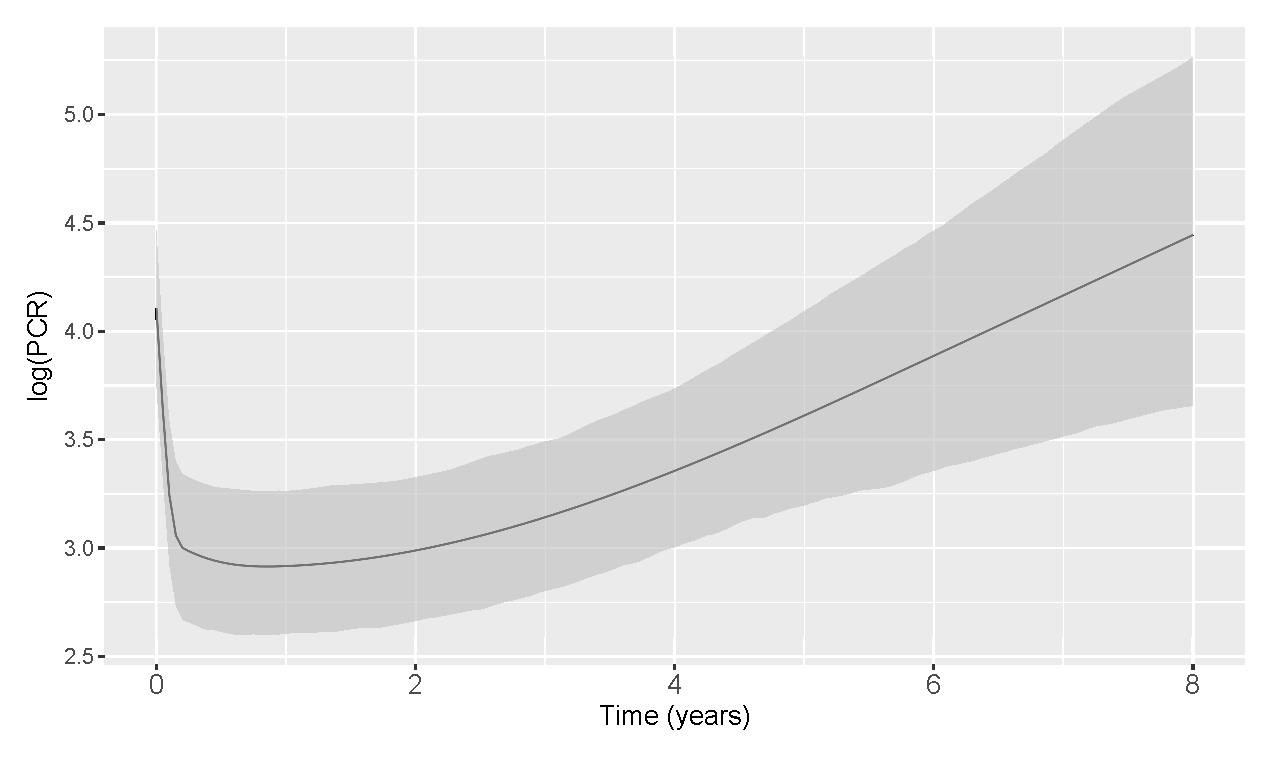
\includegraphics[width=\columnwidth]{images/pcr.eps}}
\caption{Fitted longitudinal evolution of $\log \text{PCR}$ and 95\% credible interval for a patient with the  transplantation characteristics described in Table \ref{tab : baseline_characteristics}.}
\label{fig : pcr_evolution}
\end{figure}

\begin{table}[!htb]
\begin{center}
\caption{Parameter estimates for the longitudinal sub-model for $\log \mbox{SCr}$.}
\label{tab : creatinine_long}
\begin{tabular}{lrrrrr}
\Hline
Variable                                                                         & Mean   & Std. Dev & 2.5\%  & 97.5\% & P              \\
\hline
Intercept                                                                      & 5.226  & 0.080    & 5.064  & 5.378  & \textless0.000 \\
Receiver age                                                                   & -0.063 & 0.022    & -0.107 & -0.019 & 0.010          \\
Donor age                                                                          & 0.083  & 0.020    & 0.045  & 0.119  & \textless0.000 \\
Donor BMI                                                                          & -0.011 & 0.021    & -0.054 & 0.028  & 0.612          \\
Receiver BMI                                                                         & 0.018  & 0.023    & -0.025 & 0.060  & 0.420          \\
\#HLA mismatches between donor and recipient                                                                         & 0.020  & 0.022    & -0.022 & 0.065  & 0.342          \\
Panel reactive antibody percentage                                                                          & 0.048  & 0.027    & -0.008 & 0.100  & 0.082          \\
\#Anti-hypertensive medicaments                                                                           & 0.040  & 0.020    & 0.001  & 0.080  & 0.048          \\
Cold ischemia time                                                                         & 0.029  & 0.035    & -0.039 & 0.102  & 0.390          \\
\#Days on dialysis before transplant                                                                   & 0.015  & 0.029    & -0.042 & 0.071  & 0.580          \\
Receiver gender: Male                                                                     & 0.197  & 0.042    & 0.111  & 0.276  & \textless0.000 \\
Previous transplant: Yes                                                                & 0.016  & 0.064    & -0.115 & 0.141  & 0.786          \\
Donor gender: Male                                                                      & 0.053  & 0.042    & -0.027 & 0.136  & 0.198          \\
Delayed graft function: Yes                                                                       & 0.118  & 0.049    & 0.025  & 0.216  & 0.006          \\
Diabetes Mellitus: Yes                                                                        & -0.103 & 0.059    & -0.217 & 0.012  & 0.076          \\
Cardiovascular events before transplantation: Yes                                                                     & -0.047 & 0.043    & -0.129 & 0.044  & 0.272          \\
Deceased donor: Yes                                                                 & 0.163  & 0.082    & 0.004  & 0.313  & 0.044          \\
Spline: visit time [0.039, 0.082] years & -0.440 & 0.041    & -0.517 & -0.358 & \textless0.000 \\
Spline: visit time [0.082, 0.219] years & -0.182 & 0.053    & -0.284 & -0.081 & \textless0.000 \\
Spline: visit time [0.219, 1] years & -0.545 & 0.081    & -0.712 & -0.395 & \textless0.000 \\
Spline: visit time [1, 6] years & 0.007  & 0.083    & -0.155 & 0.176  & 0.946          \\
$\sigma$                                                                            & 0.190  & 0.001    & 0.187  & 0.192  & \\
\hline
\end{tabular}
\end{center}
\end{table}

\begin{figure}[!htb]
\centerline{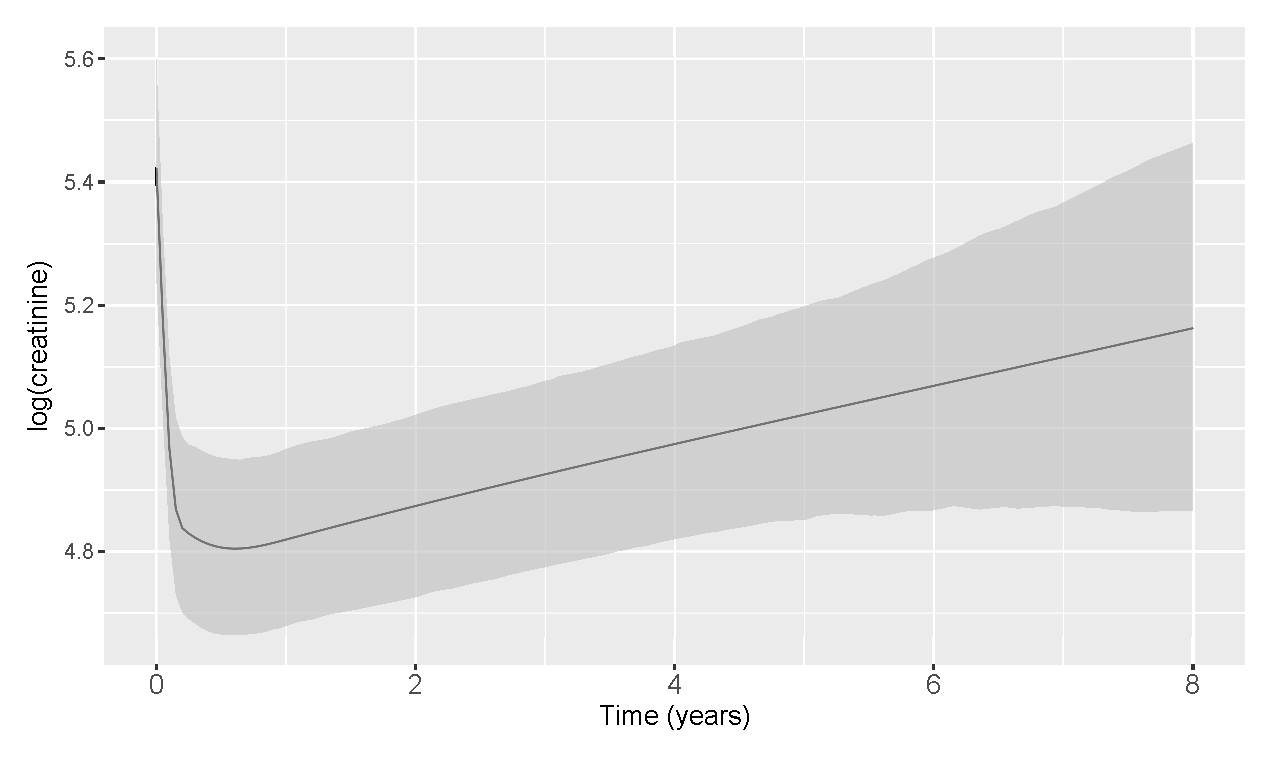
\includegraphics[width=\columnwidth]{images/creatinine.eps}}
\caption{Fitted longitudinal evolution of $\log \text{SCr}$ and 95\% credible interval for a patient with the  transplantation characteristics described in Table \ref{tab : baseline_characteristics}.}
\label{fig : creatinine_evolution}
\end{figure}

%%%%%%%%%%%%%%%%%%%%%%%%%
\clearpage
\subsection{Joint Model with Only SCr as Longitudinal Outcome}
We also fitted a joint model to the kidney transplant dataset in which only SCr was used as a longitudinal outcome. We compared this model to the joint model with both PCR and SCr outcomes using area under the receiver operating curve characteristics of the models. The results showed that the model with only SCr outcome performed as good as the model with both outcomes. Hence we used this model to create the personalized schedules for measurement of SCr levels. For this model, the parameters corresponding to the relative risk sub-model and longitudinal sub-model are presented in Table \ref{tab : relative_risk_univariate} and Table \ref{tab : creatinine_long_univariate}, respectively.

\begin{table}[!htb]
\begin{center}
\caption{Parameter estimates for the relative risk sub-model for the log hazard and 95\% credible interval. The joint model was fitted with only SCr as longitudinal outcome.}
\label{tab : relative_risk_univariate}
\begin{tabular}{lrrrrr}
\Hline
Variable               & Mean   & Std. Dev & 2.5\%  & 97.5\% & P              \\
\hline
Previous transplant: Yes      & 0.234  & 0.229    & -0.111 & 0.934  & 0.362          \\
\#HLA mismatches between donor and recipient                & 0.049  & 0.103    & -0.131 & 0.297  & 0.636          \\
Cold ischemia time                & -0.029 & 0.096    & -0.265 & 0.142  & 0.774          \\
\#Days on dialysis before transplant         & -0.016 & 0.095    & -0.229 & 0.168  & 0.918          \\
$\log \mbox{SCr}$ & 1.766  & 0.183    & 1.410  & 2.144  & \textless0.000 \\
Slope($\log \mbox{SCr}$)  & 0.261  & 0.119    & 0.040 & 0.495  & 0.010  \\
\hline
\end{tabular}
\end{center}
\end{table}


\begin{table}[!htb]
\begin{center}
\caption{Parameter estimates for the longitudinal sub-model for $\log \mbox{SCr}$. The joint model was fitted with only SCr as longitudinal outcome.}
\label{tab : creatinine_long_univariate}
\begin{tabular}{lrrrrr}
\Hline
Variable                                                                         & Mean   & Std. Dev & 2.5\%  & 97.5\% & P              \\
\hline
Intercept                                                                      & 5.250     & 0.086  & 5.083  & 5.423  & \textless0.000     \\
Receiver age                                                                    & -0.066   & 0.022  & -0.107 & -0.023 & 0.002 \\
Donor age                                                                          & 0.083    & 0.020   & 0.041  & 0.121  & \textless0.000 \\
Donor BMI                                                                           & -0.012   & 0.022  & -0.055 & 0.030   & 0.582 \\
Receiver BMI                                                                         & 0.019    & 0.023  & -0.023 & 0.061  & 0.430  \\
\#HLA mismatches between donor and recipient                                                                          & 0.018    & 0.021 & -0.023 & 0.059  & 0.424 \\
Panel reactive antibody percentage                                                                          & 0.047    & 0.027 & -0.006 & 0.101  & 0.086 \\
\#Anti-hypertensive medicaments                                                                           & 0.042    & 0.019 & 0.003  & 0.079  & 0.038 \\
Cold ischemia time                                                                         & 0.036    & 0.036 & -0.034 & 0.103  & 0.318 \\
\#Days on dialysis before transplant                                                                    & 0.014    & 0.029 & -0.047 & 0.070   & 0.582 \\
Receiver gender: Male                                                                     & 0.202    & 0.040  & 0.119  & 0.279  & \textless0.000 \\
Previous transplant: Yes                                                                 & 0.003    & 0.064 & -0.126 & 0.120   & 0.936 \\
Donor gender: Male                                                                       & 0.046    & 0.040  & -0.033 & 0.124  & 0.236 \\
Delayed graft function: Yes                                                                       & 0.118    & 0.051 & 0.021  & 0.217  & 0.020  \\
Diabetes Mellitus: Yes                                                                        & -0.101   & 0.059 & -0.214 & 0.018  & 0.102 \\
Cardiovascular events before transplantation: Yes                                                                     & -0.041   & 0.042 & -0.122 & 0.043  & 0.340  \\
Deceased donor: Yes                                                                 & 0.134    & 0.086 & -0.032 & 0.307  & 0.120  \\
Spline: visit time [0.039, 0.082] years & -0.445   & 0.041 & -0.525 & -0.365 & \textless0.000 \\
Spline: visit time [0.082, 0.219] years & -0.174   & 0.057 & -0.290  & -0.062 & \textless0.000 \\
Spline: visit time [0.219, 1] years & -0.564   & 0.085 & -0.736 & -0.409 & \textless0.000 \\
Spline: visit time [1, 6] years & -0.031   & 0.096 & -0.222 & 0.147  & 0.768 \\
$\sigma$                                                                           & 0.189    & 0.001 & 0.187  & 0.192  & \\
\hline
\end{tabular}
\end{center}
\end{table}
